\documentclass{beamer}

% Some common packages
\usepackage{graphicx, color}
\usepackage{alltt}
\usepackage{booktabs, calc, rotating}
\usepackage[round]{natbib}
\usepackage{multicol}
\usepackage{amsmath, amsbsy, amssymb, amsthm, graphicx}
\usepackage[english]{babel}
\usepackage{xkeyval} 
\usepackage{xfrac}
\usepackage[normalem]{ulem}
\usepackage{fancyvrb} 
\usepackage{tikz, geometry, tkz-graph, xcolor}
\usepackage[latin1]{inputenc}
\usepackage{times}
\usepackage[T1]{fontenc}

% Shortcuts
\newcommand{\empr}[1]{{\emph{\color{red}#1}}}
\newcommand{\cov}{\mathrm{cov}}
\newcommand{\pkg}[1]{{\textbf{\texttt{#1}}}}
\newcommand{\dif}{\mathrm{d}}
\newcommand{\bigbrk}{\vspace*{2in}}
\newcommand{\smallbrk}{\vspace*{.1in}}
\newcommand{\midbrk}{\vspace*{1in}}
\newcommand{\red}[1]{{\color{red}#1}}
\newcommand{\blue}[1]{{\color{blue}#1}}
\newcommand{\green}[1]{{\color{green}#1}}
\newcommand{\calc}[1]{{\fbox{\mbox{#1}}}}
\newcommand{\Var}{\mathrm{Var}}%
\newcommand{\Cov}{\mathrm{Cov}}%

\mode<presentation>
{
	\usetheme{UTD}
	\usecolortheme[RGB={200,0,0}]{structure}
	\setbeamercovered{transparent}
}

% fancy for Verbatim?
\fvset{frame=single,framesep=1mm,fontfamily=courier,fontsize=\scriptsize,numbers=left,framerule=.3mm,numbersep=1mm,commandchars=\\\{\}}


\title[Survival Analysis]{Applied Survival Analysis Using R\\ Chapter 11: Sample Size Determination for Survival Studies}
\author[Qi Guo]{Qi Guo}
\institute[UTD]{Department of Mathematical Sciences \\ 
	The University of Texas at Dallas}
\date{April, 19 2019}
	
\begin{document}

\begin{frame}
  \titlepage
\end{frame}

% Set up UTD backgroud
\setbeamercolor*{item}{fg=red}
\bgroup
\usebackgroundtemplate{
\tikz[overlay,remember picture] \node[opacity=0.05, at=(current page.center)] {
   
\includegraphics[height=\paperheight,width=\paperwidth]{UTDbg}};}


\section[Outline]{}
\begin{frame}
  \tableofcontents
\end{frame}

\section{Power and Sample Size for a Single Arm Study}
\begin{frame}
\frametitle{Determinate the sample size}
\begin{itemize}
\item Deciding how many subjects to include in a randomized clinical trial is a key component of its design.
\item   In survival analysis, there are two additional factors that one must specify regarding the \empr{censoring mechanism} and the \empr{particular} survival distributions.
\begin{itemize}
\item Specify what parametric survival model one is using, allows for \empr{determining the number of deaths} (or events) required to meet the power and other design specifications.
\item  Administrative reasons, provide an estimate of the number of patients that need to be entered into the trial to \empr{produce the required number of deaths}.
\end{itemize}
\end{itemize}
\end{frame}

\pagebreak
\begin{frame}
\frametitle{Hypothesis Test}
\begin{itemize}
\item The hypothesis test is $H_0: \lambda = \lambda_0$ versus $H_A:
\lambda = \lambda_A$, and the $H_0$ mean is $\mu_0 = 1/\lambda_0$ and $H_A$ mean is $\mu_A = 1/\lambda_A$, so the treatment(hazard) ratio is $\Delta = \mu_A/\mu_0 = \lambda_0/\lambda_A$. 
\item The most direct way to derive a sample size formula is based on a \empr{Wald test}, transform to let $\theta = \log(\mu) = -\log(\lambda)$, then we can express the log-likelihood function as: 
\begin{equation}
\ell(\theta) = d\log \lambda - \lambda V = -\theta d - Ve^{-\theta}
\end{equation}
and in Chapter we have shown the m.l.e $\hat{\theta} = \log(V/d)$ and $var(\hat{\theta}) \approx 1/d$, where $d = \sum\delta_i$ and $V = \sum t_i$, the number of death and total patient time.
\item So now we can use $\hat{\theta}$ as our test statistic, reject $H_0$ in favor of $H_A$ if $\hat{\theta} > k$ for some constant k.
\end{itemize}
\end{frame}

\pagebreak
\begin{frame}
\frametitle{Number of deaths to achieve}
\begin{itemize}
\item The significance level of the test, or \empr{Type I error}, is $\alpha = Pr(\hat{\theta}>k|\theta = \theta_0)$
\item Using a normalizing transformation,
\begin{equation}
Z = \frac{\hat{\theta}-\mu}{1/\sqrt{d}}
\end{equation}
so
\begin{equation}
\alpha = Pr\bigg( Z>\frac{k-\theta_0}{1/\sqrt{d}}\bigg)
\end{equation}
Hence
\begin{equation}
k = \theta_0 + \frac{z_\alpha}{\sqrt{d}}
\end{equation}
\end{itemize}
\end{frame}


\pagebreak
\begin{frame}
\frametitle{Number of deaths to achieve}
\begin{itemize}
\item The power of the test is given by:
\begin{equation}
1-\beta = Pr(\hat{\theta}>k|\theta = \theta_A) = Pr\bigg( Z>\frac{k-\theta_A}{1/\sqrt{d}}\bigg)
\end{equation}
so
\begin{equation}
-z_{\beta} = \sqrt{d} \bigg( \theta_0+ \frac{z_\alpha}{\sqrt{d}} - \theta_A\bigg)
\end{equation}
Solving for $d$ we have:
\begin{equation}
d = \frac{(z_{\beta} +z_{\alpha})^2}{(\theta_A - \theta_0)^2} = \frac{(z_{\beta} +z_{\alpha})^2}{(\log \Delta)^2}
\end{equation}
since $\log(\Delta) = \log(\lambda_0) - \log(\lambda_A)$
\item This gives us \empr{the number of deaths} needed to achieve the specified power, \empr{not the number of patients}.
\end{itemize}
\end{frame}

\pagebreak
\begin{frame}[fragile]
\frametitle{In \texttt{R}}
\begin{itemize}
\item Compute the number of deaths based on (7)
\begin{Verbatim}
> expLogMeanDeaths <- function(Delta, alpha, pwr) \{
 z.alpha <- qnorm(alpha, lower.tail=F) 
 z.beta <- qnorm(1-pwr, lower.tail=F)
 num <- (z.alpha + z.beta)^2
 denom <- (log(Delta))^2
 dd <- num/denom 
 dd   \}
\end{Verbatim}
\item We use the ``\texttt{qnorm}'' function to compute $z_\alpha$and
$z_\beta$.
\begin{Verbatim}
expLikeRatio <- function(d, alpha, pwr) \{
num <- qchisq(alpha, df=(2*d), lower.tail=F) 
denom <- qchisq(pwr, df=(2*d), lower.tail=F) 
Delta <- num/denom
Delta \}
\end{Verbatim}
\end{itemize}
\end{frame}


\section{Determining the Probability of Death in a Clinical Trial}
\begin{frame}
\frametitle{Estimate of the proportion of death}
\begin{itemize}
\item We need to provide an estimate of the proportion $\pi$ of patients who will die by the time of analysis. If all patients entered at the same time, we would simply have $\pi = 1- S(t,\lambda)$, where $t$ is the \empr{follow-up} time.
\item Patients actually enter over \empr{an accrual period} of length $a$, after accrual to the trial has ended, they are followed for an \empr{additional time} $f$. 
\item A patient who enters at time $t=0$ will have failure probability $\pi(0)=1-S(a+f,\lambda)$, so a patient who enters at time $a$, $\pi(a)=1-S(f,\lambda)$
\end{itemize}
\end{frame}

\pagebreak
\begin{frame}
\frametitle{Estimate of the proportion of death}
\begin{itemize}
\item Patients enter uniformly between times 0 and $a$, so that the patient entry follows a \empr{Uniform(0,$a$)distribution}.
\item Then the probability of death $\pi$ is obtained by averaging over these times, so that a patient that enters at time $t$ is followed for additional time $a+f-t$.
\begin{equation}
\pi = \int_{0}^{a}\frac{1}{a}Pr(death\ |\ enter\ at\ time\ t)dt
\end{equation}
or just $\mu = a+f-t $
\begin{equation}
\pi = \int_{0}^{a}\frac{1}{a}(1-S(a+f-t;\lambda))dt = 1- \frac{1}{a}\int_{a}^{a+f}S(\mu;\lambda)d\mu
\end{equation}
\item Assuming an exponential distribution, $S(\mu;\lambda) = e^{-\lambda \mu}$
\begin{equation}
\pi = 1-\frac{1}{a\lambda}\lbrace e^{-\lambda f} - e^{-\lambda(a+f)}\rbrace
\end{equation}
\end{itemize}
\end{frame}

\pagebreak
\begin{frame}[fragile]
\frametitle{In \texttt{R}}
\begin{itemize}
\item Compute the probability of death:
\begin{Verbatim}
prob.death <- function(lambda, accrual, followup) \{ 
probDeath <- 1 - (1/(accrual*lambda))* (exp(-lambda*followup) - 
exp(-lambda*(accrual + followup))) 
probDeath\}
\end{Verbatim}
\item $H_1: \lambda = 0.10$, $a = 2$ and $f=3$ years 
\begin{Verbatim}
> prob.death(lambda=0.10, accrual=2, followup=3)
[1] 0.3285622
\end{Verbatim}
\item Previously we found that 38 deaths were needed, then Then the number of patients needed is approximately $38/0.3285622=115.6$
\end{itemize}
\end{frame}

\section{Sample Size for Comparing Two Exponential Survival Distributions}
\begin{frame}
\frametitle{Prerequisites}
\begin{itemize}
\item Let $p$ denote the proportion of patients randomized to the control group, denote by $n$ the total number of patients in the trial, and we have $n_0 = np$ and $n_1 = n(1-p)$ control and experimental patients, respectively.
\item When the trial has been completed, we will observe $d_0$ and $d_1$ deaths in the control and experimental groups, and total patient times of $V_0 = \sum t_{0i}$ and $V_1 = \sum t_{1i}$.
\item The maximum likelihood estimates of the hazards $\hat{\lambda_0} = d_0/V_0$ and $\hat{\lambda_1} = d_1/V_1$. 
\item Compare the two distributions, use $\delta = \log \Delta = \log \lambda_0 - \log \lambda_1$
\end{itemize}
\end{frame}

\pagebreak
\begin{frame}
\frametitle{Number of death to achieve}
\begin{itemize}
\item Based on maximum likelihood theory
\begin{equation}
var(\hat{\delta}) = \sigma^2 = \frac{1}{n_0 \pi_0} +\frac{1}{n_1 \pi_1} = \frac{1}{np(1-p)}\cdot \frac{p\pi_0 + (1-p)\pi_1}{\pi_0 \pi_1}
\end{equation}
\item where $\pi_0$ and $\pi_1$ are the probabilities of death in the control and treatment groups, define a new
\begin{equation}
\tilde{\pi} = {\bigg( \frac{p\pi_0 + (1-p)\pi_1}{\pi_0\pi_1} \bigg) }^{-1} = {\bigg( \frac{p}{\pi_1} + \frac{1-p}{\pi_0} \bigg)}^{-1}
\end{equation}
\item $\tilde{\pi}$ is a weighted harmonic mean of $\pi_0$ and $\pi_1$
\end{itemize}
\end{frame}

\pagebreak
\begin{frame}
\frametitle{Number of death to achieve}
\begin{itemize}
\item Approximate the weighted mean $\bar{\pi} = p\pi_0 + (1-p)\pi_1$, so
\begin{equation}
var(\hat{\delta}) = \sigma^2 = \frac{1}{np(1-p)} \cdot {\tilde{\pi}}^{-1}
\end{equation}
\item Expressing the test in terms of $\delta = \log \Delta$, we reject $H_0: \delta=0$ in favor of $H_A: \delta>0$ if $\hat{\delta}>k$ for some constant k.	
\item By the similar argument before, we get $n$:
\begin{equation}
n = \frac{(z_\alpha + z_\beta)^2}{\delta^2 p(1-p)\tilde{\pi}}
\end{equation}
\item The required number of patients is the number of deaths
\begin{equation}
d = \frac{(z_\alpha + z_\beta)^2}{\delta^2 p(1-p)}
\end{equation}
\end{itemize}
\end{frame}


\section{Determining the Probability of Death from a Survival Curve Estimate}
\begin{frame}
\frametitle{Approximate}
\begin{itemize}
\item Given a survival function $\hat{S}(t)$ there are a number of ways of evaluating the integral in (9)
\item Approximate the integral by evaluating $\hat{S}(t)$ for a patient entering at time 0, $a/2$, and $a$, use some results from elementary integral calculus.
\item \empr{The trapezoidal rule}:
\begin{equation}
\pi_s \approx 1-\frac{1}{6} \big\lbrace \hat{S}(a+f) +4\hat{S}(\frac{a}{2} + f) +\hat{S}(f) \big\rbrace
\end{equation}
\item The most accurate method is to evaluate the integral numerically
\begin{equation}
\pi_r = \sum\limits_{t_{(i)}:f<t_{(i)} \le a+f}^{}[\hat{S}(a+f-t_{(i)})\cdot (t_{(i)} - t_{(i-1)})]
\end{equation}
\end{itemize}
\end{frame}

\pagebreak
\begin{frame}[fragile]
\frametitle{In \texttt{R}}
\begin{itemize}
\item Using the data ``\texttt{gastricXelox}'' from Chapter 3
\item Extract the failure times and survival probabilities:
\begin{Verbatim}
library(survival)
result.km <- survfit(Surv(timeMonths, delta) ~ 1,
conf.type="log-log") 
timesXe <- result.km$time 
survXe <- result.km$surv
\end{Verbatim}
\item Set up the accrual and follow-up times, and select the portion of the failure times in the interval from $f$ to $a+f$ 
\begin{Verbatim}
accrual <- 12
followup <- 6
times.use <- c(followup, timesXe[{timesXe >= followup} \&
{timesXe <= accrual + followup}])
surv.use <- summary(result.km, times=times.use)$surv
\end{Verbatim}
\item Finally, we use the ``\texttt{diff}'' function to get the widths of the rectangles.
\end{itemize}
\end{frame}

\pagebreak
\begin{frame}
\frametitle{In \texttt{R}}
\begin{figure}[h!]
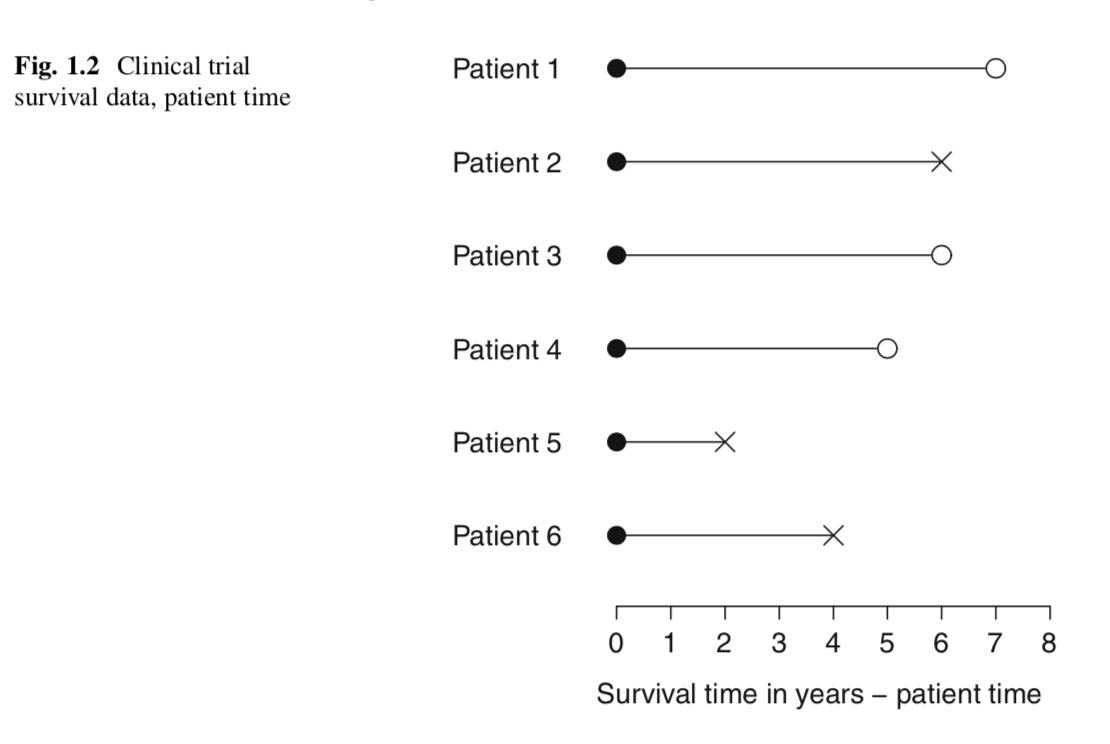
\includegraphics[scale = .5]{002.png}
\end{figure}
\end{frame}

\end{document}